\documentclass[twocolumn,prb,aps,floatfix,superscriptaddress]{revtex4-1}

\usepackage{color}
\usepackage{bm}%bold math
\usepackage{graphicx}
\usepackage{amsmath}
\usepackage{amssymb}
\usepackage{bbold}
\usepackage{setspace}
\usepackage{epstopdf}
%\usepackage{scalerel}
\epstopdfsetup{update} % only regenerate pdf files when eps file is newer
\linespread{1}
\usepackage[export]{adjustbox}

%\newcommand*\bplqt{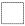
\includegraphics[height=1.6ex] {Symbols/blank_plqt}}
%\newcommand*\bhrzmv{\includegraphics[height=1.6ex]{Symbols/blank_hrzmv}}
%\newcommand*\bdiag{\includegraphics[height=1.6ex] {Symbols/blank_diag}}
%\newcommand*\bstr{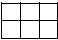
\includegraphics[height=1.6ex] {Symbols/blank_str}}

\newcommand{\figref}[1]{Fig. \ref{#1}}
\newcommand{\secref}[1]{Sec. \ref{#1}}
\newcommand{\tabref}[1]{Tab. \ref{#1}}
\newcommand{\note}[1]{\textcolor{red}{#1}}

%\newcommand*{\hprs}{%
%  \text{% change size in subscripts or superscripts
%    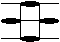
\includegraphics[
%      height=1.2ex,% adjust to suit
%      valign=M,% center vertically
%      raise=\fontdimen22\textfont2,% but raise it to the formula axis
%    ]{Symbols/hrzprestar} }
%}
%\newcommand*{\hspr}{%
%  \text{% change size in subscripts or superscripts
%    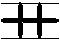
\includegraphics[
%      height=1.2ex,% adjust to suit
%      valign=M,% center vertically
%      raise=\fontdimen22\textfont2,% but raise it to the formula axis
%    ]{Symbols/hrzstarpair} }
%}

\newcommand*{\bplqt}{%
  \text{% change size in subscripts or superscripts
    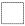
\includegraphics[
      height=1.2ex,% adjust to suit
      valign=M,% center vertically
      raise=\fontdimen22\textfont2,% but raise it to the formula axis
    ]{Symbols/blank_plqt} }
}
\newcommand*{\fplqt}{%
  \text{% change size in subscripts or superscripts
    
\includegraphics[
      height=1.2ex,% adjust to suit
      valign=M,% center vertically
      raise=\fontdimen22\textfont2,% but raise it to the formula axis
    ]{Symbols/full_plqt} }
}
%\newcommand*{\bhrzmv}{%
%  \text{% change size in subscripts or superscripts
%    \includegraphics[
%      height=1.2ex,% adjust to suit
%      valign=M,% center vertically
%      raise=\fontdimen22\textfont2,% but raise it to the formula axis
%    ]{Symbols/blank_hrzmv} }
%}
%\newcommand*{\bdiag}{%
%  \text{% change size in subscripts or superscripts
%    \includegraphics[
%      height=1.2ex,% adjust to suit
%      valign=M,% center vertically
%      raise=\fontdimen22\textfont2,% but raise it to the formula axis
%    ]{Symbols/blank_diag} }
%}
%\newcommand*{\bstr}{%
%  \text{% change size in subscripts or superscripts
%    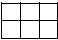
\includegraphics[
%      height=1.2ex,% adjust to suit
%      valign=M,% center vertically
%      raise=\fontdimen22\textfont2,% but raise it to the formula axis
%    ]{Symbols/blank_str} }
%}
\newcommand*{\vvemptylink}{%
  \text{% change size in subscripts or superscripts
    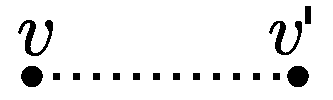
\includegraphics[
      height=1.8ex,% adjust to suit
      valign=M,% center vertically
      raise=\fontdimen22\textfont2,% but raise it to the formula axis
    ]{Symbols/string_net_link_sym0} }
}
\newcommand*{\emptylink}{%
  \text{% change size in subscripts or superscripts
    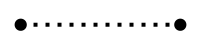
\includegraphics[
      height=1.5ex,% adjust to suit
      valign=M,% center vertically
      raise=\fontdimen22\textfont2,% but raise it to the formula axis
    ]{Symbols/string_net_link_sym1} }
}
\newcommand*{\rightarrowlink}{%
  \text{% change size in subscripts or superscripts
    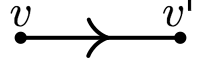
\includegraphics[
      height=1.5ex,% adjust to suit
      valign=M,% center vertically
      raise=\fontdimen22\textfont2,% but raise it to the formula axis
    ]{Symbols/string_net_link_sym2} }
}
\newcommand*{\leftarrowlink}{%
  \text{% change size in subscripts or superscripts
    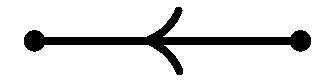
\includegraphics[
      height=1.5ex,% adjust to suit
      valign=M,% center vertically
      raise=\fontdimen22\textfont2,% but raise it to the formula axis
    ]{Symbols/string_net_link_sym3} }
}
\newcommand*{\twointwoout}{%
  \text{% change size in subscripts or superscripts
    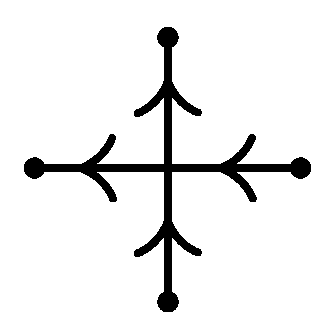
\includegraphics[
      height=1.5ex,% adjust to suit
      valign=M,% center vertically
      raise=\fontdimen22\textfont2,% but raise it to the formula axis
    ]{Symbols/two_in_two_out} }
}
\newcommand*{\oneinoneout}{%
  \text{% change size in subscripts or superscripts
    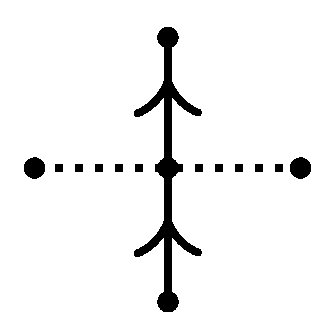
\includegraphics[
      height=1.5ex,% adjust to suit
      valign=M,% center vertically
      raise=\fontdimen22\textfont2,% but raise it to the formula axis
    ]{Symbols/one_in_one_out} }
}
\newcommand*{\threeinzeroout}{%
  \text{% change size in subscripts or superscripts
    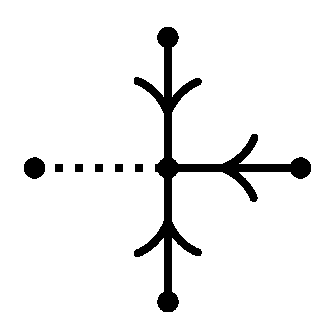
\includegraphics[
      height=1.5ex,% adjust to suit
      valign=M,% center vertically
      raise=\fontdimen22\textfont2,% but raise it to the formula axis
    ]{Symbols/three_in_zero_out} }
}
\newcommand*{\threeoutzeroin}{%
  \text{% change size in subscripts or superscripts
    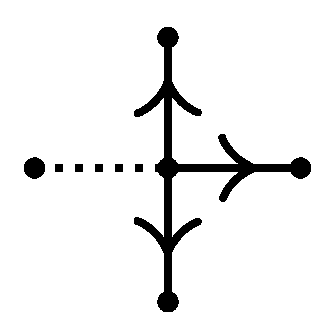
\includegraphics[
      height=1.5ex,% adjust to suit
      valign=M,% center vertically
      raise=\fontdimen22\textfont2,% but raise it to the formula axis
    ]{Symbols/three_out_zero_in} }
}
\newcommand*{\zerooutzeroin}{%
  \text{% change size in subscripts or superscripts
    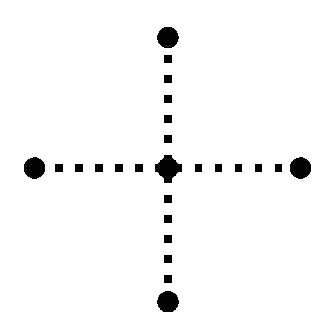
\includegraphics[
      height=1.5ex,% adjust to suit
      valign=M,% center vertically
      raise=\fontdimen22\textfont2,% but raise it to the formula axis
    ]{Symbols/zero_out_zero_in} }
}
\newcommand*{\hrzplqt}{%
  \text{% change size in subscripts or superscripts
    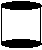
\includegraphics[
      height=1.5ex,% adjust to suit
      valign=M,% center vertically
      raise=\fontdimen22\textfont2,% but raise it to the formula axis
    ]{Symbols/hrzplqt.pdf} }
}
\newcommand*{\vrtplqt}{%
  \text{% change size in subscripts or superscripts
    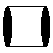
\includegraphics[
      height=1.5ex,% adjust to suit
      valign=M,% center vertically
      raise=\fontdimen22\textfont2,% but raise it to the formula axis
    ]{Symbols/vrtplqt.pdf} }
}
%\newcommand*{\threedownplqt}{%
%  \text{% change size in subscripts or superscripts
%    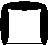
\includegraphics[
%      height=1.5ex,% adjust to suit
%      valign=M,% center vertically
%      raise=\fontdimen22\textfont2,% but raise it to the formula axis
%    ]{Symbols/threedownplqt.pdf} }
%}
%\newcommand*{\threeupplqt}{%
%  \text{% change size in subscripts or superscripts
%    
\includegraphics[
%      height=1.5ex,% adjust to suit
%      valign=M,% center vertically
%      raise=\fontdimen22\textfont2,% but raise it to the formula axis
%    ]{Symbols/threeupplqt.pdf} }
%}
%\newcommand*{\threerightplqt}{%
%  \text{% change size in subscripts or superscripts
%    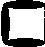
\includegraphics[
%      height=1.5ex,% adjust to suit
%      valign=M,% center vertically
%      raise=\fontdimen22\textfont2,% but raise it to the formula axis
%    ]{Symbols/threerightplqt.pdf} }
%}
\newcommand*{\threeleftplqt}{%
  \text{% change size in subscripts or superscripts
    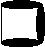
\includegraphics[
      height=1.5ex,% adjust to suit
      valign=M,% center vertically
      raise=\fontdimen22\textfont2,% but raise it to the formula axis
    ]{Symbols/threeleftplqt.pdf} }
}
%\newcommand*{\onedownplqt}{%
%  \text{% change size in subscripts or superscripts
%    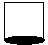
\includegraphics[
%      height=1.5ex,% adjust to suit
%      valign=M,% center vertically
%      raise=\fontdimen22\textfont2,% but raise it to the formula axis
%    ]{Symbols/onedownplqt.pdf} }
%}
%\newcommand*{\oneupplqt}{%
%  \text{% change size in subscripts or superscripts
%    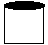
\includegraphics[
%      height=1.5ex,% adjust to suit
%      valign=M,% center vertically
%      raise=\fontdimen22\textfont2,% but raise it to the formula axis
%    ]{Symbols/oneupplqt.pdf} }
%}
%\newcommand*{\onerightplqt}{%
%  \text{% change size in subscripts or superscripts
%    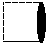
\includegraphics[
%      height=1.5ex,% adjust to suit
%      valign=M,% center vertically
%      raise=\fontdimen22\textfont2,% but raise it to the formula axis
%    ]{Symbols/onerightplqt.pdf} }
%}
\newcommand*{\oneleftplqt}{%
  \text{% change size in subscripts or superscripts
    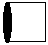
\includegraphics[
      height=1.5ex,% adjust to suit
      valign=M,% center vertically
      raise=\fontdimen22\textfont2,% but raise it to the formula axis
    ]{Symbols/oneleftplqt.pdf} }
}
\newcommand*{\twoupplqt}{%
  \text{% change size in subscripts or superscripts
    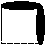
\includegraphics[
      height=1.5ex,% adjust to suit
      valign=M,% center vertically
      raise=\fontdimen22\textfont2,% but raise it to the formula axis
    ]{Symbols/twoupplqt.pdf} }
}
\newcommand*{\twodownplqt}{%
  \text{% change size in subscripts or superscripts
    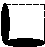
\includegraphics[
      height=1.5ex,% adjust to suit
      valign=M,% center vertically
      raise=\fontdimen22\textfont2,% but raise it to the formula axis
    ]{Symbols/twodownplqt.pdf} }
}
\newcommand*{\svrtmon}{%
  \text{% change size in subscripts or superscripts
    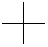
\includegraphics[
      height=3.5ex,% adjust to suit
      valign=M,% center vertically
      raise=\fontdimen22\textfont2,% but raise it to the formula axis
    ]{Symbols/sing_vrt_monomer.pdf} }
}
\newcommand*{\svrtdmr}{%
  \text{% change size in subscripts or superscripts
    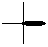
\includegraphics[
      height=3.5ex,% adjust to suit
      valign=M,% center vertically
      raise=\fontdimen22\textfont2,% but raise it to the formula axis
    ]{Symbols/sing_vrt_dimer.pdf} }
}
\newcommand*{\svrttrmr}{%
  \text{% change size in subscripts or superscripts
    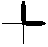
\includegraphics[
      height=3.5ex,% adjust to suit
      valign=M,% center vertically
      raise=\fontdimen22\textfont2,% but raise it to the formula axis
    ]{Symbols/sing_vrt_trimer.pdf} }
}
\newcommand*{\svrttrmrtwo}{%
  \text{% change size in subscripts or superscripts
    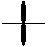
\includegraphics[
      height=3.5ex,% adjust to suit
      valign=M,% center vertically
      raise=\fontdimen22\textfont2,% but raise it to the formula axis
    ]{Symbols/sing_vrt_trimer2.pdf} }
}
\newcommand*{\svrtquat}{%
  \text{% change size in subscripts or superscripts
    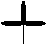
\includegraphics[
      height=3.5ex,% adjust to suit
      valign=M,% center vertically
      raise=\fontdimen22\textfont2,% but raise it to the formula axis
    ]{Symbols/sing_vrt_quatramer.pdf} }
}
\newcommand*{\svrtpent}{%
  \text{% change size in subscripts or superscripts
    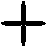
\includegraphics[
      height=3.5ex,% adjust to suit
      valign=M,% center vertically
      raise=\fontdimen22\textfont2,% but raise it to the formula axis
    ]{Symbols/sing_vrt_pentamer.pdf} }
}
\newcommand*{\pentmvcreate}{%
  \text{% change size in subscripts or superscripts
    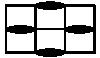
\includegraphics[
      height=3.5ex,% adjust to suit
      valign=M,% center vertically
      raise=\fontdimen22\textfont2,% but raise it to the formula axis
    ]{Symbols/pentmvcreate1.pdf} }
}
\newcommand*{\pentmvanal}{%
  \text{% change size in subscripts or superscripts
    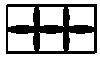
\includegraphics[
      height=3.5ex,% adjust to suit
      valign=M,% center vertically
      raise=\fontdimen22\textfont2,% but raise it to the formula axis
    ]{Symbols/pentmvcreate2.pdf} }
}
\newcommand*{\penmvhrzleft}{%
  \text{% change size in subscripts or superscripts
    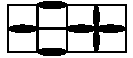
\includegraphics[
      height=3.5ex,% adjust to suit
      valign=M,% center vertically
      raise=\fontdimen22\textfont2,% but raise it to the formula axis
    ]{Symbols/pentmvhorzleft.pdf} }
}
\newcommand*{\penmvhrzright}{%
  \text{% change size in subscripts or superscripts
    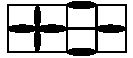
\includegraphics[
      height=3.5ex,% adjust to suit
      valign=M,% center vertically
      raise=\fontdimen22\textfont2,% but raise it to the formula axis
    ]{Symbols/pentmvhorzright.pdf} }
}
\newcommand*{\penmvdiagup}{%
  \text{% change size in subscripts or superscripts
    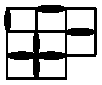
\includegraphics[
      height=5.5ex,% adjust to suit
      valign=M,% center vertically
      raise=\fontdimen22\textfont2,% but raise it to the formula axis
    ]{Symbols/pentmvdiagup.pdf} }
}
\newcommand*{\penmvdiagdown}{%
  \text{% change size in subscripts or superscripts
    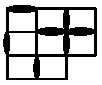
\includegraphics[
      height=5.5ex,% adjust to suit
      valign=M,% center vertically
      raise=\fontdimen22\textfont2,% but raise it to the formula axis
    ]{Symbols/pentmvdiagdown.pdf} }
}
\newcommand*{\monomermvA}{%
  \text{% change size in subscripts or superscripts
    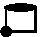
\includegraphics[
      height=3.5ex,% adjust to suit
      valign=M,% center vertically
      raise=\fontdimen22\textfont2,% but raise it to the formula axis
    ]{Symbols/monomer_mv_1} }
}
\newcommand*{\monomermvB}{%
  \text{% change size in subscripts or superscripts
    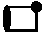
\includegraphics[
      height=3.5ex,% adjust to suit
      valign=M,% center vertically
      raise=\fontdimen22\textfont2,% but raise it to the formula axis
    ]{Symbols/monomer_mv_2} }
}
\newcommand{\ket}[1]{| #1 \rangle}
\newcommand{\eket}[1]{\left | #1 \right \rangle}
\newcommand{\ebra}[1]{\left \langle #1 \right |}
\newcommand{\Eqref}[1]{Eq. \eqref{#1}}
\newcommand{\RK}{\mathrm{RK}}
\newcommand{\HGQDM}{H_\mathrm{GQDM}}
\newcommand{\HQDM}{H_\mathrm{QDM}}
\newcommand{\HIGT}{H_\mathrm{IGT}}
\newcommand{\HQDPM}{H_\mathrm{QDPM}}

%%%%%%%%%%%%%%%%%%%%%%%%%%%%%%%%%%%%%%%%%%%%%%%%%%%%%%%%%%%%%%%%%%%%%%%%%%%%%%%%%%%%%%%%%%%%%%%
\begin{document}

\title{$Z_3$ topological order in the quantum dimer-pentamer model}

\author{Owen Myers}
\email{omyers@uvm.edu}
\affiliation{Department of Physics, University of Vermont, Burlington, VT 05405, USA}

\author{C. M. Herdman}
\affiliation{Institute for Quantum Computing, University of Waterloo, Ontario, N2L 3G1, Canada}
\affiliation{Department of Physics \& Astronomy, University of Waterloo, Ontario, N2L 3G1, Canada}
\affiliation{Department of Chemistry,  University of Waterloo, Ontario, N2L 3G1, Canada}

\begin{abstract}
We study the ground state of the quantum dimer-pentamer model (QDPM) on the square lattice. This model is a generalization of the square lattice quantum dimer model (QDM) as its configuration space comprises fully-packed hard-core dimer coverings as well as configurations containing pentamers, where four dimers touch a vertex. Thus in the QDPM, the fully-packed, hard-core constraint of the QDM is relaxed such that the local dimer number at each vertex is fixed modulo 3; correspondingly, the local $U(1)$ gauge symmetry of the QDM Hilbert space is reduced to a local $Z_3$ gauge symmetry in the QDPM. We construct a local Hamiltonian for which the Rokhsar-Kivelson (RK) state (the equal superposition of all configurations in a topological sector) is the exact ground state and has a 9-fold topological degeneracy on the torus. Using Monte Carlo calculations, we find no spontaneous symmetry breaking in the RK wavefunction and that its dimer-dimer correlation function decays exponentially. Additionally, we discuss the possibility of $Z_3$ topological order in the ground state of the QDPM.
\end{abstract}

\maketitle

%%%%%%%%%%%%%%%%%%%%%%%%%%%%%%%%%%%%%%%%%%%%%%%%%%
\section{Introduction}
%%%%%%%%%%%%%%%%%%%%%%%%%%%%%%%%%%%%%%%%%%%%%%%%%%

Over the last several decades, experimental and theoretical work has demonstrated that strongly interacting quantum many-body systems support exotic quantum phases of matter not described by the Landau symmetry breaking paradigm. One class of such quantum phases of matter are topologically ordered quantum liquids~\cite{Wen1990}, first realized experimentally via the fractional quantum Hall effect~\cite{Tsui1982,Laughlin1983,Wen1990a,Wen1995}. Despite the absence of conventional symmetry breaking and a local order parameter, topological quantum liquids possess a non-trivial quantum order that distinguishes them from trivial liquid phases~\cite{Nayak2008}. Although not detectable by local operators, topological order arises due to a non-local entanglement structure that leaves a signatures in the bipartite entanglement entropy~\cite{Levin2006a,Kitaev2006b}. Such topological phases may provide the basis for fault-tolerant quantum information processing~\cite{Freedman2001,Kitaev2003}.

Because of the exotic nature of topological phases and their potential use for quantum information processing, there is great interest in the development of theoretical models which display these phases. Such models offer the possibility of furthering the understanding of these phases as well as providing candidate experimental systems in which to constructively engineer topological order~\cite{Duan2003,Jaksch2005,Lewenstein2007,Jiang2008d,Weimer2010a,Herdman2010c,Fowler2012a}. A variety of exactly soluble lattice models are known to support ground states with topological order that ranges from the simplest variety, $Z_2$ topological order~\cite{Kitaev2003,Wen2003}, to those with non-Abelian anyonic excitations~\cite{Levin2005a,Kitaev2006a}; such models generally involve complex many-body interactions, and thus it is desirable to find simpler models supporting topological order that are closer to what is accessible experimentally.

Among the simplest class of models displaying topological quantum liquid phases are those with local geometric constraints; the constraints inhibit the formation of symmetry breaking local order and given sufficient dynamics, may lead to a symmetric liquid ground state. One of the most basic of these is the quantum dimer model (QDM) describing dimer degrees of freedom living on the links of a lattice~\cite{Rokhsar1988,Moessner2008}; the hard-core, fully-packed QDM has a local constraint that requires exactly one dimer touching each vertex.

%%%%%%%%%%%%%%%%%%%%%%%%%%%%
\begin{figure}[t!]
    \centering
    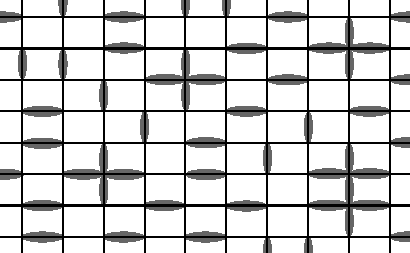
\includegraphics[width=0.75\columnwidth]{QDPM_ex_config.pdf}
    \caption{An example of an allowed configuration in the quantum dimer-pentamer model, in which pentamers (four dimers touching at a vertex) are allowed. \note{Owen: maybe we should stick with black and white for these cartoons}}
    \label{fig:QDPMex}
\end{figure}
%%%%%%%%%%%%%%%%%%%%%%%%%%%%

While on non-bipartite lattices, the QDM posses a topologically ordered ground state~\cite{Moessner2001a,Fendley2002}, on the square lattice there is only a liquid ground state at an isolated critical quantum point~\cite{Leung1996,Syljuasen2006}. If the hard-core constraint of the QDM is relaxed to a parity constraint such that each vertex much have an odd (or even) number of dimers touching each vertex, the simplest non-trivial dynamics leads to a $Z_2$ topologically ordered ground state~\cite{Kitaev2003,Wen2003}. The existence of topologically ordered ground states in dimer-based models is intimately related to the local constraint which imposes a local gauge symmetry in the Hilbert space; the topological order that arises is directly related to a discrete gauge theory with the appropriate local gauge constraint~\cite{Moessner2001}.

Given that these models with dimer degrees of freedom and local constraints posses the simplest non-trivial local (Ising) Hilbert space at each link, they provide a potentially simpler route to engineering exotic phases. The local constraints can often be enforced by a local potential energy penalty and the required dynamics are generally expected to arise at the lowest order non-trivial order in perturbation theory. We will refer to such models with dimer degrees of freedom on links and local constraints at vertices as \emph{generalized quantum dimer modes} (GQDMs). Previous work as demonstrated that GQDMs on the square lattice support gapped $Z_2$ topologically ordered phases as well as gapless quantum critical points. On non-bipartite lattices, GQDMs support $Z_2$ topological order~\cite{Moessner2001a,Misguich2002} as well as doubled-semion phases~\cite{Qi2014,Buerschaper2014a}. A full characterization of all exotic phases that can exist within this framework is thus desirable.

In this work we extend this paradigm to a new GQDM on the square lattice, what we term the \emph{quantum dimer-pentamer model} (QDPM). In the QDPM, the local constraint is relaxed from that of the QDM to allow either $1$ or $4$ dimers to touch each vertex, as shown in figure \figref{fig:QDPMex}. Correspondingly, the QDPM extends the Hilbert space of the QDM to include both fully-packed hard-core dimer configurations, as well as those with pentamers--four dimers touching a vertex. To give the system dynamics, the Hamiltonian includes terms that incorporate the simplest non-trivial dynamics that preserve the local constraint.

We present a numerical study of the ground state of the QDPM at an exactly soluble point and demonstrate the the soluble point represents a \textcolor{red}{gapped}, disordered quantum liquid phase.  Using Monte Carlo calculations, we explicitly demonstrate the absence of symmetry breaking order and the exponential decay of correlation functions; \textcolor{red}{by computing imaginary-time correlation functions, we find that the RK point is gapped in the thermodynamic limit}. By construction the QDPM has an exact local $Z_3$ symmetry and conserves a $Z_3$ topological winding number. Thus the QDPM has a 9-fold topological degeneracy on the torus. Thus we argue that the ground state of the QDPM posses $Z_3$ topological order.

This this paper is organized as follows. In \secref{sec:Background} we provide relevant background for the QDM and related models. In \secref{sec:QDPM} we present the details of the QPDM. \secref{sec:MC} provides the results of a Monte Carlo study of the ground state of the QDPM at its exactly soluble point.


%%%%%%%%%%%%%%%%%%%%%%%%%%%%%%%%%%%%%%%%%%%%%%%%%%
\section{Background}
\label{sec:Background}
%%%%%%%%%%%%%%%%%%%%%%%%%%%%%%%%%%%%%%%%%%%%%%%%%%

%%%%%%%%%%%%%%%%%%%%%%%%%%%%%%%%%%%%%%%%%%%%%%%%%%
\subsection{Generalized quantum dimer models}
\label{sec:GQDM}

%%%%%%%%%%%%%%%%%%%%%%%%%%%%
\begin{figure}[htpb]
    \centering
    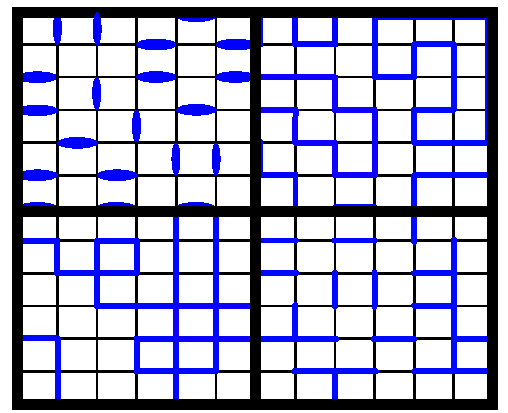
\includegraphics[width=0.8\linewidth]{example_local_constraints.pdf}
    \caption{Clockwise from the upper left panel we show an example of a QDM with constraints: one
    dimer ($n_0 = 1$), two dimers ($n_0 = 2$), and an even ($n_P = 0$) or odd ($n_P = 1$) number of dimers touching each vertex. \note{Owen: Maybe for consistency we should make all the dimers loos like the dimers in the upper-left.}}
    \label{fig:example_local_constraints}
\end{figure}
%%%%%%%%%%%%%%%%%%%%%%%%%%%%
Here we will provide background about generalized quantum dimer models on the square lattice. We consider systems with Ising-like dimer degrees of freedom on each link, such that each link has either $0$ or $1$ dimers. Given an Ising spin $\sigma_\ell$ on each link $\ell$ we define the number of dimers on the link $n_\ell \equiv 1/2+\sigma_\ell^z$, where $\sigma_\ell^i$ are the associated Pauli matrices. The Hilbert space consists of configurations of dimers on the square lattice that satisfy a local constraint at each vertex. We define a $U(1)$ charge $Q_v$ at each vertex $v$ of the lattice in terms of the number of dimers touching $v$, $n_v\equiv \sum_{\ell \in v}n_\ell$:
\begin{equation}
Q_v \equiv \pm \left( n_v - c_P \right)
\end{equation}
where $c_P = 2$, ($c_P=1$) for models in the even (odd) sector of the constraint, and the $+$($-$) sign corresponds to vertices on the $A$($B$) sublattice. A local dimer number constraint requires $Q_v$ to vanish for all vertices; a dimer parity constraint requires only $(Q_v\mod 2)$ to vanish.
 
The Hamiltonian of a GQDM is of the form
\begin{equation}
H_{\rm{GQDM}} = -\sum_\nu t_\nu \hat{T}_{\nu} + \sum_\nu v_\nu \hat{V}_{\nu} \label{eq:HGQDM}
\end{equation}
where $\hat{T}_\nu$ are off-diagonal kinetic energy operators, $\hat{V}_\nu$ are diagonal the potential energy operators, $t_\nu$ and $v_\nu$ parametrize the strength of these terms, and each $\nu$ and represents a set of $n_\nu$ neighboring links. We will limit our discussion to $t_\nu >0$. $\hat{T}_\nu$ is constructed to favor a resonance between two distinct allowed dimerazations of $\nu$, $c_\nu$ and its compliment $\bar{c}_\nu$, and is written as:
\begin{equation}
\hat{T}_{\nu} = \eket{c_\nu}\ebra{\bar{c}_\nu} + h.c.;
\end{equation}
in the simplest case, $\hat{T_\nu}$ involves the minimum non-trivial dimer dynamics that preserve the constraint. Similarly, the potential energy term provides an energy cost for states with these local configurations:
\begin{equation}
\hat{V}_{\nu} = \eket{c_\nu}\ebra{c_\nu} +  \eket{\bar{c}_\nu}\ebra{\bar{c}_\nu}.
\end{equation}
Therefore we may define a Hamiltonian for a GQDM using \Eqref{eq:HGQDM} and defining a set of dimer resonances $\{(c_\nu,\bar{c}_\nu)\}$ and corresponding potential and kinetic energy strenghts $\{(t_\nu,v_\nu)\}$:
\begin{equation}
\HGQDM \biggl( \bigl\{\left(c_\nu,\bar{c}_\nu\right)\},\{\left(t_\nu,v_\nu\right)\bigr\}\biggr).
\end{equation}
 In general the $T_\nu$'s don't commute with each other or with the $V_\nu$'s, and thus the ground state of $H_{\rm{GQDM}}$ is not explicitly known.

However, at the special points in the $\{(t_\nu,v_\nu)\}$ parameter space, the exact ground state is known when \Eqref{eq:HGQDM} can be written as the sum of projection operators
\begin{equation}
H_{\rm{RK}} = \sum_\nu \hat{h}_\nu \label{eq:HRK},
\end{equation}
where all $h_\nu$ are projectors with eigenvalues $\{0,1\}$; a zero energy ground state of \Eqref{eq:HRK} is simultaneously annihilated by all $\hat{h}_\nu$. Such a zero energy state, known as the RK state, may be formed from an equal superposition of all dimerizations that are connected by $\{T_\nu\}$:
\begin{equation}
\eket{\Phi_{\RK}^{\Omega}} = \sum_{C \in \Omega} \eket{C}
\end{equation} 
where $\Omega$ is a subset of the Hilbert space connected by $\{T_\nu\}$. Thus $\{ \ket{\Phi_{\RK}^\Omega} \}$ are the exact, degenerate ground states of $H_{\rm{GQDM}}$ with a degeneracy labelled by $\Omega$ at the RK point.

Because of the local constraints, all states $\ket{\psi}$ in the Hilbert space of a GQDM are invariant under local gauge transformations $G_v \ket{\psi} = \ket{\psi}$ a the vertices, $G_v$ of the general form~\cite{Moessner2001}
\begin{equation}
G_v = e^{i \alpha_v Q_v}, \label{eq:Gv}
\end{equation}
where the allowed values of $\alpha_v$ depend on the constraint.  
By construction, the Hamiltonian is gauge invariant and thus commutes with $G_v$
\begin{equation}
\left[ H_{\rm{GQDM}}, G_v \right] = 0. \notag
\end{equation}

If a defect is introduced which violates the local constraint at a vertex, this can be viewed as an ``electric charge'' living on the vertex, within the context of the original GQDM. 
%Defects may be created in a GQDM by defining an ``electric string'' operator that creates pairs of defects and thus generating ``charged'' states that are outside the gauge invariant Hilbert space:
%\begin{equation}
%S_{vv'}^e \equiv \prod_{\ell \in \tilde{\gamma}_{vv'}} \sigma_\ell^x
%\end{equation}
%where $\tilde{\gamma}_{vv'}$ is an open string on the lattice from $v$ to $v'$. When acting on a gauge invariant state, $S_{\tilde{\gamma}}^e$ creates a neutral pair of charges $Q_v = \pm 1$ at the ends of $\tilde{\gamma}$ where the signs depend on the lattice and the initial configuration of vertices.
One may determine if such electric charges are confined by introducing a pair of such defects and computing their spatial correlation function, thus determining the confined or deconfined nature of the GQDM ground state.

The gauge symmetry allows one to construct a gauge invariant string operator $S_\gamma$ along an oriented path $\gamma$ path on the dual lattice. We first orient all the links of the square lattice such that they point from the $A$ sublattice to the $B$ sublattice (see \figref{fig:orientedSL}) and define an oriented dimer flux $\Phi_\gamma$ through the path:
\begin{equation}
\Phi_\gamma \equiv \sum_{\ell \in \gamma} \rm{sgn}\left(\ell,\gamma\right) n_\ell \label{eq:phi}
\end{equation}
where $\mathrm{sgn}(\ell,\gamma)$ is positive (negative) if $\ell$ is oriented to the right with respect to the orientation of $\gamma$. Additionally, we define background flux $\tilde{\Phi}_\ell$
\begin{equation}
\tilde{\Phi}_\gamma \equiv - \sum_{\ell \in \gamma} \rm{sgn}\left(\ell,\gamma\right) \tilde{n}_\ell \label{eq:phiBackground}
\end{equation}
where $n_\ell$ is the number operator for a static background dimer configuration which is chosen to fix the gauge, and the total charge enclosed in a closed loop $\Gamma$ is $Q_\Gamma = \Phi_\Gamma+ \tilde{\Phi}_\Gamma$. (Alternately can think of the source of $\tilde{\Phi}_\Gamma$ to be static charges of charge $+c_0$ ($-c_0$) sitting at the verticies of the $A$($B$) sub-lattice.).

We define the string operator is defined as
\begin{equation}
S_\gamma \left( \alpha \right) \equiv e^{i \alpha \left( \Phi_\gamma - \tilde{\Phi}_\gamma \right)} \label{eq:Sgamma}
\end{equation}
where $\alpha$ such that $S_\gamma$ commutes with $\HGQDM$ everywhere except at the ends of $\gamma$. Therefore, for closed loops $\Gamma$, $[ S_\Gamma,\HGQDM]=0$. For open strings, $S_\gamma$ does not commute with the Hamiltonian and can be viewed as creating a pair of ``magnetic charges'' at the ends of the string: correspondingly $S_\gamma \ket{\Phi_{\RK}}$ can used as a trial wavefunction for an excited state with a pair of magnetic vortices. If a state has topological order with deconfined electric charges, these magnetic vortices should be gapped excitations, and correspondingly the magnetic string operator should decay exponentially~\cite{Read1989a,Senthil2000,Senthil2001e}. The condensation of magnetic vortices can drive a phase transition from a topologically ordered phase to a conventionally order phase~\cite{Jalabert1991,Ralko2007,Huh2011}. Thus, the magnetic string correlation can be used as test for deconfinement of electric charges.

On surfaces with non-trivial topology, we may define the topological loop operators
\begin{equation}
W_{X,Y} \left( \alpha \right) \equiv S_{\Gamma_{X,Y}} \left( \alpha \right)
\end{equation}
where $\Gamma_{X,Y}$ are topologically non-trivial closed loops that wind once about the $X$ and $Y$ directions of the torus, respectively. Since $W_{X,Y} (\alpha)$ commute with the Hamiltonian, we may use their eigenvalues to label the ground states.

%%%%%%%%%%%%%%%%%%%%%%%%%%%%
\begin{figure}[tpb]
    \centering
    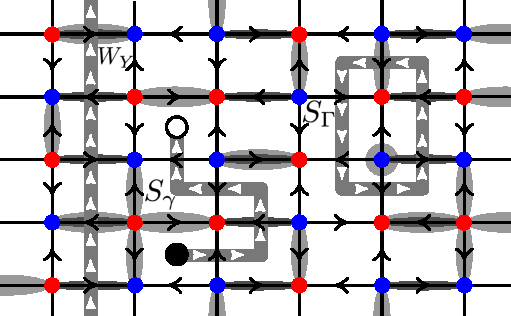
\includegraphics[width=1.0\columnwidth]{mag_loops_on_orntd_lat.pdf}
    \caption{$\Phi_i$: a nontrivial string winding around the system in one of the two possible
        directions. $\Phi_2$: an open
    magnetic string with two different charged (colored) visons at the end points. $\Phi_3$ a trivial closed
    string. The colors red and blue distinguish the two different sublattices that orient the links.}
    \label{fig:orientedSL}
\end{figure}
%%%%%%%%%%%%%%%%%%%%%%%%%%%%

%%%%%%%%%%%%%%%%%%%%%%%%%%%%
\subsection{Fixed dimer number constraints}

The two unique fixed-number constraints on the square lattice are lead to QDM in the odd sector and the quantum full-packed loop model (QFPLM) in the even sector. For configurations that satisfy these a number constraints, $Q_v$ strictly vanishes, and thus all states in the Hilbert space are invariant under $G_v$ for $0 \leq \alpha_v \leq 2 \pi$ in \Eqref{eq:Gv}; this represents a local $U(1)$ gauge symmetry. 

The Hamiltonian for these models gives dynamics to parallel dimers on the plaquettes $\bplqt$ of the lattice:
\begin{equation}
\HQDM\left(t,v\right) \equiv \HGQDM \biggl( \bigl\{ \left(\vrtplqt,\hrzplqt\right) \bigr\},\bigl\{ \left(t,v\right) \bigr\} \biggr)  \label{eq:HQDM}
\end{equation}
where we have taken $t_\bplqt = t$ \& $v_\bplqt =v$ $\forall \bplqt$.
%\begin{align}
%    \label{}
%   \HQDM = &-t\sum_{\bplqt} \biggl( \eket{\vrtplqt} \ebra{\hrzplqt} +h.c. \biggr) \notag\\
%    					&+v\sum_{\bplqt} \biggl( \eket{\vrtplqt} \ebra{\vrtplqt} +\eket{\hrzplqt} \ebra{\hrzplqt} \biggr). \label{eq:HQDM}
%\end{align}
In this case of a fixed number constraint, the Hamiltonian conserves $Q_v$ and therefore the dimer flux through any closed loop such that:
\begin{equation}
\left[ \Phi_\Gamma, \HQDM \right] = 0
\end{equation}
and therefore we can define two conserved topological winding numbers $\Phi_{x}$ \& $\Phi_{y}$ which are the dimer flux through topologically non-trival loops that wind around each axis of the lattice when the system has periodic conditions (see \figref{fig:orientedSL}). On an lattice of dimensions $L_x\times L_y$, the the eigenvalues of $\Phi_{x/y}$ integers in range	
\begin{equation}
-L_{x/y}/2 \leq  \Phi_{x/y} \leq L_{x/y}/2,
\end{equation}
thus there are $\mathcal{O} (L_x L_y)$ distinct topological sectors. 

At the Rokhsar-Kivelson point $t=v$, we may write $\HQDM$ in the form of \Eqref{eq:HRK} by defining projection operators  $\hat{h}_\nu \equiv \hat{P}^\dagger_{\nu} \hat{P}_{\nu}$, with
\begin{equation}
\hat{P}^\dagger_\nu \equiv \biggl( \eket{ c_\nu} - \eket{\bar{c}_\nu} \biggr).
\end{equation} 
Since the plaquette flip term in \Eqref{eq:HQDM} is ergodic in each of topological sector $(\Phi_x,\Phi_y)$ on the square lattice (\textcolor{red}{is this known for the FPLM???})~\cite{????}, each topological sector corresponds to a unique RK ground state where $\Omega$ is labeled by $(\Phi_x,\Phi_y)$. Thus the equal superposition RK points of the QDM and QFPLM have an \emph{extensively} degenerate ground states.

Defects in these models correspond to states with $Q_v \neq 0$; a table of the charges associated with defects in the QDM and QFPLM is listed in \tabref{tab:defects}.

The QDM and QFPLM on the square lattice have isolated liquid ground states at the RK point surrounded by symmetry broken phases~\cite{Rokhsar1988,Leung1996,Syljuasen2005,Syljuasen2006,Syljuasen2004,Moessner2008}. The RK point of these models have been shown to have power-law decaying dimer-dimer and monomer-monomer correlation functions and gapless excitations~\cite{Fisher1961,Kasteleyn1961,Fisher1966a,Fisher1963,Kasteleyn1963a,Sutherland1988b,Sutherland1988a,Kohmoto1988a,Liang1988,Sutherland1988,Kohmoto1988,Levitov1990,Leung1996,Henley1997,Henley1997,Henley2004a,Pollmann2006}. Thus, such fixed number constrained models on bipartite lattices are expected to have an isolated unstable gapless critical quantum liquid points with logarithmically confined defect and an extensive topological degeneracy. These features of fixed number constrained models are consistent with the effective U(1) gauge theory description of the RK point~\cite{Fradkin2004,Fradkin1990,Moessner2001}; in 2+1D pure U(1) gauge theories are always confining and thus the lack of an extended deconfined topologically ordered phase near the RK point~\cite{PolyakovBook}.

%%%%%%%%%%%%%%%%%%%%%%%%%%%%
\begin{table}
  \begin{tabular}{| l | c | c | c | c | c |}
  	\hline
    %type & $n_v$ & $Q_v^{\rm{QDM}}$ & $Q_v^{\rm{FPLM}}$  & $Q_v^{Z_3}$ & \\
    type & $n_v$ & $Q_v^{\rm{QDM}}$ & $Q_v^{\rm{FPLM}}$  & $Q_v^{QDPM}$ & \\
	\hline
    monomer & $0$ & -1 & -2 &  -1 & $\svrtmon$  \\
	\hline
    dimer & $1$ & 0 & -1 &   0 & $\svrtdmr$ \\
	\hline
    trimer & $2$ & 1 & 0 &   1 & $\svrttrmr$ $\svrttrmrtwo$ \\
	\hline
    tetramer & $3$ & 2 & 1 &   -1 & $\svrtquat$ \\
	\hline
    pentamer & $4$ & 3 & 2 &  0 & $\svrtpent$  \\
	\hline
  \end{tabular}
  \caption{Defects where $n_v$ dimers touch a vertex and their associated $U(1)$ charges on the A sub-lattice in both the QDM, QFPLM, and QDPM. Defects on the B sub-lattice have opposite charge.}
  \label{tab:defects}
\end{table}
%%%%%%%%%%%%%%%%%%%%%%%%%%%%


%%%%%%%%%%%%%%%%%%%%%%%%%%%%
\subsection{Fixed dimer parity constraints}

We now consider relaxing the local constraint to a parity constraint such that only $Q_v^{Z_2} \equiv (Q_v \mod 2)$ is required to vanish; the resulting GQDM are the even and odd sectors are the  even \& odd Ising gauge theories (IGT) (and the closely related even and odd sector Toric Codes). In these cases, the local constraint requires $\alpha_v \in \{ 0, \pi\}$ in \Eqref{eq:Gv} and therefore the gauge symmetry is reduced from $U(1)$ to $Z_2$. The set of allowed dimer resonances $\mathcal{C}_{\rm{TC}}$ is expanded accordingly:
\begin{align}
\mathcal{C}_{\rm{TC}} &\equiv \bigl\{ \left(c_{\Box,i},\bar{c}_{\Box,i}\right) \bigr\} \\
&=\bigl\{
\left(\vrtplqt,\hrzplqt\right),\left(\threeleftplqt,\oneleftplqt\right),\left(\twodownplqt,\twoupplqt\right),\left(\bplqt,\fplqt\right) \bigr\}
\end{align}
where we implicitly include rotational symmetry related resonances. We will limit or discussion to $v_\bplqt=0$ such that the corresponding Hamiltonian is
\begin{equation}
\HIGT\left(t\right) \equiv \HGQDM \biggl( \mathcal{C}_{\rm{IGT}},\bigl\{ \left(t,0\right) \bigr\} \biggr).
\end{equation}
In this case the equal superposition RK wavefunction is the exact ground state occurs in the absence of a potential energy term, as we can define a projection operator on each plaquette
\begin{equation}
h_\Box \equiv \frac{1}{2} \left( \mathbb{1} - \sum_i \eket{c_{\Box,i}}\ebra{\bar{c}_{\Box,i}} + h.c. \right)
\end{equation}
such that $\HIGT$ takes the form of \Eqref{eq:HRK} (up to a constant), and the RK state is the ground state for all values of $t$.

The increased dynamics of $\HIGT$ vs. $\HQDM$ no longer conserve the dimer flux $\Phi_\Gamma$ through a closed curve; only $\Phi_\Gamma \mod 2$ is preserved by $\HIGT$. Consequently, to define the string and loop operators which commutes with $\HIGT$ (for closed strings) we fix $\alpha = \pi$ in \Eqref{eq:Sgamma}:
\begin{equation}
S_\gamma^{\rm{IGT}} \equiv S_\gamma \left( \pi \right), \quad W_{X,Y}^{\rm{IGT}} \equiv W_{X,Y} \left( \pi \right).
\end{equation}
Thus the $W_{X,Y}^{\rm{IGT}}$ have two eigenvalues $\pm 1$, and the topological sectors on the torus can be labeled as $\Omega: (\pm 1,\pm1)$; consequently the extensive degeneracy of the fixed number constrained models has been reduced to a finite ground state degeneracy in the fixed parity models.

Defects in the Ising Gauge theories have $Q_v^{Z_2} = 1$ and we identify these defects as $Z_2$ electric charges on the corresponding vertices. 

The ground states of $\HIGT$ are fourfold degenerate on the torus and have exponentially decaying dimer-dimer and monomer-monomer correlations (\textcolor{red}{Is this known for both sectors}) and a finite energy gap; such features demonstrated the deconfined topologically ordered nature of the ground state of the IGTs.

We may understand the emergence of the $Z_2$ topologically ordered phase of IGTs from the QDM and QFPLM from the following picture. The additional vertex configurations that are allowed in the IGTs (monomers and pentamers in the even sector and tetramers in the odd sector) relative to the number constrained models have $Q_v = \pm 2$. It is known that coupling a $U(1)$ gauge field to a charge $q$ matter field can result in an $Z_q$ gauge theory~\cite{Fradkin1979}; thus in the IGTs we have addded dynamic charge 2 defects to the underlying $U(1)$ symmetric model, and we may expect a $Z_2$ gauge theory to result. We note that pentamers are charge $\pm3$ objects in the QDM (see \tabref{tab:defects}); thus below we investigate whether introducing pentamers into the QDM leads to an effective $Z_3$ gauge theory.


%%%%%%%%%%%%%%%%%%%%%%%%%%%%%%%%%%%%%%%%%%%%%%%%%%%%%%%%%%%%%%%%%%%%%%%%%%%%%%%%%%%%%%%%%%%%%%%
%%%%%%%%%%%%%%%%%%%%%%%%%%%%%%%%%%%%%%%%%%%%%%%%%%%%%%%%%%%%%%%%%%%%%%%%%%%%%%%%%%%%%%%%%%%%%%%
\section{The Quantum Dimer Pentamer Model}

We define the Hilbert space of the QDPM to be an odd sector GQDM where vertices are constrained to be touched by a single dimer or the center of a pentamer, such that $n_v = 1,4$. For defect-free configurations in the QDPM, $Q_v$ only vanishes modulo $3$;  thus we may define a $Z_3$ charge,
\begin{equation}
Q_v^{Z_3} \equiv \left(Q_v~\rm{mod}~3\right)
\end{equation}
 which strictly vanishes at each vertex, representing the local constraint. All states in the QDPM are invariant under an exact local $Z_3$ gauge symmetry given by \Eqref{eq:Gv} with $\alpha_v \in \{0,\pm 2\pi/3\}$. Thus introducing pentamers in the QDM reduces the gauge symmetry from $U(1)$ to $Z_3$.

The Hamiltonian of the QDPM is defined by \Eqref{eq:HGQDM} including both plaquette flips as well as local dimer resonances that create and destroy pairs of pentamers, and allow single pentamers to translate on the same sub-lattice (see \tabref{tab:pentamer_moves}). Thus we may write $\HQDPM$ as the following:
\begin{equation}
\HQDPM \equiv \HQDM + H_{\rm{pent}}
\end{equation}
where $H_{\rm{pent}}$ only involves the resonances in \tabref{tab:pentamer_moves} involving pentamers. 
 
\begin{table}
    \begin{tabular}{| l | c | c |}
  	\hline
     & $c$ & $\bar{c}$ \\
	\hline
    $i$ & $\pentmvcreate$ &  $\pentmvanal$  \\
	\hline
    $ii$ &$\penmvhrzleft$&$\penmvhrzright$ \\
	\hline
    $iii$ &$\penmvdiagup$& $\penmvdiagdown$\\
	\hline
  \end{tabular}
  \caption{The pairs of local dimer \& pentamer configurations $c\leftrightarrow\bar{c}$ generate minimal local dynamics that create/annihilate pairs ($i$) of pentamers and translate single pentamers ($ii$ \& $iii$). Note that pentamers always stay on the same sublattice which is associated with their $U(1)$ charge. }
  \label{tab:pentamer_moves}
\end{table}
 
Because of the terms involving pentamers, $\HQDPM$ conserves $Q_v^{Z_3}$ rather than $Q_v$, and thus $\Phi_\Gamma$ does not commute with the Hamiltonian for closed loops $\Gamma$. The appropriate string and loop operator corresponds to \Eqref{eq:Sgamma} with $\alpha = 2\pi/3$:
\begin{equation}
S_\gamma^{\rm{QDPM}} \equiv S_\gamma \left( 2\pi/3\right), \quad W_{X,Y}^{\rm{QDPM}} \equiv W_{X,Y} \left( 2\pi/3\right). \label{eq:SQDPM}
\end{equation}
Thus we have 
\begin{equation}
\left[ W_{X,Y}^{\rm{QDPM}}, \HQDPM \right] = 0.
\end{equation}
and for closed curves $\Gamma$
\begin{equation}
\left[ S_\Gamma^{\rm{QDPM}}, \HQDPM \right] = 0.
\end{equation}

Our numerical simulations (discussed below in \secref{sec:numerics}) suggest that the dynamics of $\HQDPM$ are ergodic in each topological sector. The exact zero energy ground state at the RK point, where $t_i=v_i, i \in \{ 0,1,2,3\}$, is the RK state, where the superposition is taken to be over all states in the topological sector $\Omega$ which are labeled by the topological loop operators
\begin{equation}
\Omega = \left(W_X^{\rm{QDPM}},W_Y^{\rm{QDPM}} \right)
\end{equation}
Since the $W_{X,Y}^{\rm{QDPM}}$ operators have eigenvalues $\{0,1,-1\}$...

Defects in the QDPM (monomers, trimers, and tetramers) carry a $Z_3$ electric charge $Q_v^{Z_3} = \pm 1$, where the sign depends on the sub-lattice and type of defect (see \ref{tab:defects}).

Thus we have demonstrated that ground state at the RK point of the QDPM has an exact $Z_3$ gauge symmetry and a corresponding $9$-fold topological degeneracy on the torus. We emphasize that despite the exact $Z_3$ local gauge symmetry of the QDPM, there is not an exact mapping to a $Z_3$ gauge theory on the square lattice, as the QDPM has Ising degrees of freedom on the links, rather than the 3 dimensional local Hilbert space of a $Z_3$ gauge theory.  It remains to address whether this RK state is in the deconfined $Z_3$ topologically ordered phase of a $Z_3$ gauge theory, or a critically correlated or confining symmetry broken phase, which we do below.


%%%%%%%%%%%%%%%%%%%%%%%%%%%%%%%%%%%%%%%%%%%%%%%%%%%%%%%%%%%%%%%%%%%%%%%%%%%%%%%%%%%%%%%%%%%%%%%
%%%%%%%%%%%%%%%%%%%%%%%%%%%%%%%%%%%%%%%%%%%%%%%%%%%%%%%%%%%%%%%%%%%%%%%%%%%%%%%%%%%%%%%%%%%%%%%
\section{Numerical Study of the RK ground state of the QDPM}
\label{sec:numerics}

To determine the nature of the ground state at the RK point of the QDPM, we have used Monte Carlo sampling of $\ket{\Psi_{\rm{RK}}}$, using local updates corresponding to the dimer resonances shown in \tabref{tab:pentamer_moves} to compute ground state expectation values. Below we present the results of calculations on $L\times L$ lattices with periodic boundary conditions on systems up to $L=64$. 

%%%%%%%%%%%%%%%%%%%%%%%%%%%%%%%%%%%%%%%%%%%%%%
\subsection{Topological sectors}

We explicitly demonstrate how the extensive topological degeneracy of the QDM is reduced to a finite degeneracy in the QDPM by computing the histogram of $U(1)$ topological winding number $\Phi_X$ . This is shown in \figref{fig:u1_wind_qdpm}, where the different colors represent calculations that were initialized to different winding sectors; we confirm that $\Phi_{X/Y}$ is only conserved modulo $3$, rather than strictly conserved as it is in the QDM. We find that $P(\Phi_{X/Y})$ has a roughly gaussian envelope with a width that scales with system size--this is expected as $\Phi_{X/Y} = \pm L/2$ correspond to ordered configurations and thus there are fewer dimer configurations near these limits. Thus we find that the QDPM has a \emph{finite} $9$-fold degeneracy on the torus, where the topological sectors are labeled by $\Phi_{X/Y} \mod 3$, or equivalently $(W_X^{\rm{QDPM}},W_Y^{\rm{QDPM}})$, in contrast with the extensive degeneracy of the QDM. Additionally, we find no evidence of a lack of ergodicity within each of the 9 topological sectors. For the remainder of the paper we present results in the $(0,0)$, topological sector, but we see no dependence the topological sector for any of the results presented here~\note{Owen: which calculations/system sizes have you checked different topological sectors?}.
%%%%%%%%%%%%%%%%%%%%%%%
\begin{figure}[]
    \centering
    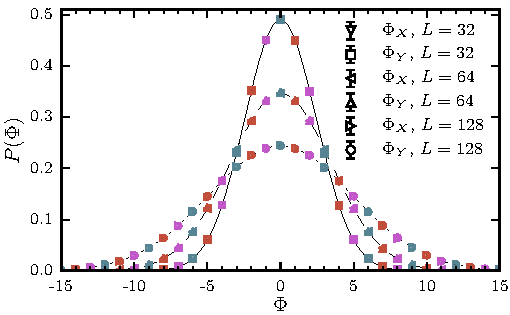
\includegraphics[width=1.0\linewidth]{u1_wind_qdpm.pdf}
    \caption{The histogram of the $U(1)$ winding number $\Phi_X$ as measured in the QDPM on a
    $L=32$ lattice. Different colors correspond to calculations initialized to different winding sectors. Note that $\Phi_X$ is conserved modulo $3$, resulting in a $9$-fold topological degeneracy on a torus.
    \note{Owen: change the y-axis label to $P(\Phi_x)$ and the x-axis to $\Phi_x$. Is this still an $L=32$ lattice? Do you have $L=64$? Perhaps put both on the same plot? (with no vertical bars)}}
    \label{fig:u1_wind_qdpm}
\end{figure}
%%%%%%%%%%%%%%%%%%%%%%%


%%%%%%%%%%%%%%%%%%%%%%%%%%%%%%%%%%%%%%%%%%%%%%
\subsection{Dimer density correlations}

Here we discuss the dimer density correlations in the RK ground state of the QDPM. In \figref{fig:dimer_vison_heatmap} we plot the bare dimer-dimer density correlation function $\langle n_{\bm{0}} n_{\bm{r}}\rangle$ on an $L=16$ lattice; here the origin $\bm{0}$ represents the blue link, and $\bm{r}$ varies over all other links of the lattice. We see no evidence of symmetry breaking in the dimer correlations on lattices up $L=64$. We will restrict the rest of our disucssion to correlations between horizontal of dimers, as we find no rotational symmetry breaking, or qualitative difference between the the correlations between parallel dimers and perpendicular dimers.

%%%%%%%%%%%%%%%%%%%%%%%
    \begin{figure}
        \centering
        \includegraphics[width=1.0\columnwidth]{dimer_gry_scale_qdpm.pdf}
        \caption{({\it left}) Gray scale of the dimer-dimer correlation function $\langle n_{\bm{0}} n_{\bm{r}}\rangle$ on an $L=16$ lattice. The origin corresponds to the blue link, and $\bm{r}$ varies over all other links of the lattice. Red links have correlations that are off the given scale.~\note{Owen: Is this the bare or connected correlation function? What do these plots look like on a log scale?} ({\it right}) The $Z_3$ magnetic string correlation function $C_m(\bm{r}_{\bm{0}p})$, where the the correlations is with respect to the blue plaquette. \note{Are we using the real part? What does $\sqrt{C_M^*C_m}$ look like? Regardless we should make this a positive quantity so the lefthand side of the grayscale is zero.}}
        \label{fig:dimer_vison_heatmap}
    \end{figure}
%%%%%%%%%%%%%%%%%%%%%%%

The left panel of \figref{fig:structure_factor} shows the equal-time dimer-dimer structure factor, 
\begin{equation}
S_d\left( \bm{k} \right) \equiv \frac{1}{ L^2} \sum_{i,j} e^{-i \bm{k} \cdot \left(\bm{r}_i - \bm{r}_j\right)} \left \langle n_i n_j \right \rangle
\end{equation}
where we restrict the sum to horizontal links, for an $L=32$ lattice. $S_d(\bm{k})$ displays maxima at $\bm{k} = (0, \pm \pi)$ due to correlation between parallel links on a given plaquette but we see no evidence of translational symmetry breaking. The lack of rotational symmetry of $S_d(\bm{k})$ is due to the fact that we have isolated horizontal dimers--we see no evidence of rotational symmetry breaking between horizontal and vertical dimer correlations. \figref{fig:structure_factor_path} shows $S_d(\bm{k})$ for a particular path through the Brillouin zone.

%%%%%%%%%%%%%%%%%%%%%%%
   \begin{figure}[]
        \centering
        \includegraphics[width=1.0\columnwidth]{qdpm_dmr_vis_HM_16x16.pdf}
        \caption{({\it left}) The horizontal dimer density structure factor $S_d(\bm{k})$ for the QDPM RK ground state on an $L=32$ lattice. The lack of $x\leftrightarrow y$ rotational symmetry is due to the fact that horizontal links have been isolated. ({\it right}) \note{Owen: Is this the real part or $\sqrt{S_M^* S_M}$}}
        \label{fig:structure_factor} 
    \end{figure}
%%%%%%%%%%%%%%%%%%%%%%%
%%%%%%%%%%%%%%%%%%%%%%%
    \begin{figure}[]
        \centering
        \includegraphics[width=1.0\columnwidth]{vis_dmr_qdpm_struc_fac_32x32.pdf}
        \caption{ The horizontal dimer-dimer structure factor $S_d(\bm{k})$ ({\it top}) and the $Z_3$ magnetic string structure factor $S_M$ ({\it bottom})
        shown along the path in $k$ space connecting the $(0,0)$, to $(\pi,0)$, $(\pi,\pi)$, $(0,0)$
        points for $\gamma=0.5$. Statistical errors are smaller than the symbols. \note{Owen: Make the k's in the y-axis bold. What do there look like if you added $L=16$ data to these plots? Switch the y-axis from $S_v\rightarrow S_M$.}}
        \label{fig:structure_factor_path}
    \end{figure}
%%%%%%%%%%%%%%%%%%%%%%%
%%%%%%%%%%%%%%%%%%%%%%%

Additionally we have studied the nature of the decay of the connected dimer-dimer correlation function,
  \begin{equation}
    C_{\mathrm{d}} \left(r\right) \equiv \langle n_{\bm{0}} n_{\bm{r}} \rangle - \langle n_{\bm{0}} \rangle   \langle n_{\bm{r}} \rangle   
\end{equation}
where $r$ is the distance between the links $\bm{0}$ and $\bm{r}$. In \figref{fig:spatial_dmr_cor}, $C_d$ between parallel links is plotted as a function of separation, \textcolor{red}{for both $r$ parallel and perpendicular to the orientation of the dimers} \note{(Owen: can you add both directions to this plot?)} for an $L=64$ lattice. We find that $C_d$ decays exponentially with distance with a correlations length  $\chi\approx???$; additionally we find that correlations between perpendicular dimers also decay exponentially.

Thus we find that the RK point of the QDPM is a symmetric dimer liquid with exponentially decaying dimer correlations, in contrast with the power-law decaying correlations of the 

%%%%%%%%%%%%%%%%%%%%%%%
\begin{figure}
    \centering
    \includegraphics[width=1.0\columnwidth]{spatial_cors_parallel.pdf}
    \caption{The dimer-dimer density correlation function $C_d$ between parallel links in the QDPM RK ground state on a $L=64$ lattice, in directions perpendicular (circles) and parallel (squares) to the dimer orientation.  The lines represent the best fit to an exponential decay with correlation length $\chi\approx???$. \note{Owen: Can you add the other direction to this plot? The y-axis also needs a label. Can you add the correlation length estimate here as well? Can you add the $r=0$ data point to this plot?}}
    \label{fig:spatial_dmr_cor}
\end{figure}
%%%%%%%%%%%%%%%%%%%%%%%

%%%%%%%%%%%%%%%%%%%%%%%%%%%%%%%%%%%%%%%%%%%%%%
\subsection{$Z_3$ magnetic string correlations}

To investigate the $Z_3$ gauge theory description of the QDPM RK ground state, we study the $Z_3$ magnetic string correlation function as defined in \eqref{eq:Sgamma} \& \eqref{eq:SQDPM}:
\begin{equation}
C_M \left( \bm{r}_{pp'} \right) \equiv \left \langle \exp \left[ \frac{2 \pi}{3} i \left( \Phi_{\gamma_{pp'}} -\tilde{\Phi}_{\gamma_{pp'}} \right) \right] \right \rangle
\end{equation}
where $p$ and $p'$ are two plaquettes, and $\gamma_{pp'}$ is any open string on the dual lattice connecting $p$ and $p'$. \note{Something about the background dimerization and gauge fixing here. Are we using the real parts or $\sqrt{C_M^*C_M}$?}

In \figref{fig:dimer_vison_heatmap}, we have ploted $C_M$ for an $L=16$ lattice, which displays short distance correlations that quickly decay. \note{Comment here about gauge fixing breaking symmetry, if still present...}. Additionally, we have plotted the magnetic string structure factor
\begin{equation}
S_M\left( \bm{k} \right) \equiv \frac{1}{ L^2} \sum_{p,p'} e^{-i \bm{k} \cdot r_{pp'}} C_M\left( \bm{r}_{pp'}\right)
\end{equation}
in \figref{fig:structure_factor}. \note{Discuss any effect of gauge fixing here, if relevant}. 

\figref{fig:vison_cor} show the decay of $C_M$ along one of the axes of the dual lattice; \note{we find this decays exponentially with distance, with a correlation length $\chi\approx???$} 

Thus we find no evidence of magnetic vortex condensation on lattices up to $L=64$.

%%%%%%%%%%%%%%%%%%%%%%%
\begin{figure}
    \centering
    \includegraphics[width=1.0\columnwidth]{spatial_cors_z3_vis.pdf}
    \caption{ $Z_3$ magnetic string correlation $C_M$ along along one axis of an $L=64$ lattice. The line corresponds to an exponential fit with correlations length \note{$\chi\approx???$}.}
    \label{fig:vison_cor}
\end{figure}
%%%%%%%%%%%%%%%%%%%%%%%



%%%%%%%%%%%%%%%%%%%%%%%%%%%%%%%%%%%%%%%%%%%%%%
\subsection{Monomer deconfinement}

To study the confinement of electrically charged defects in the QDPM, we have Monte Carlo sampled the RK ground state doped with a single pair of monomers. We initialize the system with a monomer on each sub-lattice and supplement the local Monte Carlo updates with updates of the form:
\begin{equation}
\monomermvA  \Longleftrightarrow \monomermvB
\end{equation}
which appear to provide ergodic dynamics in the monomer-dimer-pentamer configuration space. Notice that monomers remain on the same sub-lattice, which is consistent with their assignment of a $Z_3$ electric charge of $\pm1$, where the positive and negative monomers live on different sub-lattices. 

We then can test for the confinement of monomers by studying the monomer-monomer density correlation function $\langle m_{\bm{0}} m_{\bm{r}} \rangle$, which is plotted in \figref{fig:monomer_correlation}. If the monomers are confined, we expect $\langle m_{\bm{0}} m_{\bm{r}} \rangle$ to decay to zero at large distances; conversely if monomers are deconfined, we expect the monomers to be randomly distributed on the lattice, such that $\langle m_{\bm{0}} m_{\bm{r}} \rangle \sim L^{-4}$ at large separations. In \figref{fig:monomer_correlations}, the horizontal lines correspond to $L^{-4}$ for each system size; we find that the monomer correlations quickly decay to $L^{-4}$ indicating a deconfinement of monomers.

%%%%%%%%%%%%%%%%%%%%%%%
    \begin{figure}[]
        \centering
        \includegraphics[width=1.0\columnwidth]{monomer_cor_log.pdf}
        \caption{ The monomer-monomer correlations function $\langle m_{\bm{0}} m_{\bm{r}} \rangle$ along a coordinate axis in the QDPM RK ground state doped with a single pair of monomers on lattices up to \note{$L=48$}. The horizontal lines correspond to $L^{-4}$ for the system size corresponding to the color. \note{Owen: Do you have data for $L=64$? Can you make the subscripts in the y-axis label bold math? Maybe we should renomalize this plot by a factor of $L^2$. This is only one sub-lattice--what about the other sublattice?}}
        \label{fig:monomer_correlations}
    \end{figure}
%%%%%%%%%%%%%%%%%%%%%%%
%%%%%%%%%%%%%%%%%%%%%%%

%%%%%%%%%%%%%%%%%%%%%%%%%%%%%%%%%%%%%%%%%%%%%%%%%%%%%%%%%%%%%%%%%%%%%%%%%%%%%%%%%%%%%%%%%%%%%%%
%%%%%%%%%%%%%%%%%%%%%%%%%%%%%%%%%%%%%%%%%%%%%%%%%%%%%%%%%%%%%%%%%%%%%%%%%%%%%%%%%%%%%%%%%%%%%%%
\section{Discussion}

We have introduced the quantum dimer-pentamer model on the square lattice and studied the ground state at the RK point. Using numerical calculations, we have demonstrated that the RK state of the QDPM is a dimer liquid, without spontaneously broken symmetry. The extensive topological degeneracy of the square lattice QDM has been reduced to a finite 9-fold degeneracy in the QDPM on a torus. We find that the dimer correlations decay exponentially with distance in contrast to the power-law decay of dimer correlations in the QDM. Additionally we also have demonstrated that monomer defects are deconfined in the QDPM, in contrast with the critical confinement of monomers in the QDM. Finally, we find that the $Z_3$ magnetic string correlations decay exponentially and display no evidence of $Z_3$ vortex condensation; this is consistent with $Z_3$ vortices being gapped quasiparticles excitations above the QDPM ground state. 

The above results suggest a the low energy physics of the QDPM is described by a $Z_3$ gauge theory with a $Z_3$ topological ordered ground state. Thus we have demonstrated that systems with Ising degrees of freedom and local constraints can lead to $Z_N$ topological order for $N>2$, providing the a new stable phase of matter beyond the commonly seen $Z_2$ topological spin liqud.

Future work could directly probe the existence of a finite gap above the RK point by studying the imaginary time dynamics of correlations functions using Monte Carlo methods similar to those used in here~\cite{Henley1997,Henley2004a}; such an approach could be used to explore if the low energy excitations are best described by $Z_3$ magnetic vorticies~\cite{Ivanov2004,Ralko2007,Misguich2008d}. Additionally, one could conclusively demonstrate the existence of $Z_3$ topological order by computing the topological entanglement entropy in the QDPM ground state Monte Carlo methods~\cite{Levin2005a,Kitaev2006b,Hastings2010}. 

A finite gap above the RK point suggests that a stable topologically ordered phase should exist surrounding the RK point. While the Monte Carlo techniques used in this manuscript are limited to the RK point, the phase diagram near the RK point can be explored in future work using quantum Monte Carlo methods, as the QDPM has no sign problem. Away from RK, the condensation of $Z_3$ magnetic vortices could drive a continuous phase transition out of the topologically order phase, analogous to vison condensation in $Z_2$ spin liquids~\cite{Jalabert1991,Ralko2007,Huh2011,Hao2014,Slagle2014}; if such a continuous transition exists in the QDPM it may provide access to a new universality of class of quantum transitions~\cite{XU2012}.

Finally, given the stability of the topologically ordered phase, it may be possible to realize the QDPM in a more microscopically realistic spin model with two body interactions. The local constraints of the QDM can be realized in two-body spin-$1/2$ and Bose-Hubbard models, and the QDM Hamiltonian can arise perturbatively in the constrained low energy Hilbert space~\cite{Balents2002a,Zhitomirsky2005,Isakov2006c,Albuquerque2008}. Thus future work, it may be possible to engineer the QDPM in the low energy subspace of an experimentally realizable two-body model.

%%%%%%%%%%%%%%%%%%%%%%%%%%%%%%%%%%%%%%%%%%%%%%%%%%%%%%%%%%%%%%%%%%%%%%%%%%%%%%%%%%%%%%%%%%%%%%%
%%%%%%%%%%%%%%%%%%%%%%%%%%%%%%%%%%%%%%%%%%%%%%%%%%%%%%%%%%%%%%%%%%%%%%%%%%%%%%%%%%%%%%%%%%%%%%%
\section{Acknowledgements}

Our calculations were performed on the VACC....

%%%%%%%%%%%%%%%%%%%%%%%%%%%%%%%%%%%%%%%%%%%%%%%%%%%%%%%%%%%%%%%%%%%%%%%%%%%%%%%%%%%%%%%%%%%%%%%
%%%%%%%%%%%%%%%%%%%%%%%%%%%%%%%%%%%%%%%%%%%%%%%%%%%%%%%%%%%%%%%%%%%%%%%%%%%%%%%%%%%%%%%%%%%%%%%
\appendix

    \section{$Z_3$ Toric Code on the Square Lattice}
        In the $Z_3$ toric three degrees of freedom live on each link.
        We can represent the $Z_3$ algebra through the following expressions
        %
        %Z_N
        %\begin{equation}
        %    E |n\rangle = n |n\rangle, ~ n=0,1,2,...,N-1
        %    \\
        %    e^{iA} |n\rangle = |n+1 \rangle, ~ n=0,1,2,...,N-2
        %    \\
        %    e^{iA} |N-1\rangle = |0\rangle
        %    %\label{eqn:}
        %\end{equation}
        %Z_3
        %
        \begin{equation}
            \begin{split}
            & E_l |n_l\rangle = n_l |n_l\rangle, ~ n_l=0,1,2
            \\
            & e^{iA_l} |n_l \rangle = |n_l+1 \rangle, ~ n_l =0,1
            \\ 
            & e^{iA_l} |2 \rangle = |0\rangle
            \end{split}
            ,
            %\label{eqn:}
        \end{equation}
        %
        where the operators $E_l$ and $A_l$ act on a given link $l$ and are analogous to the 
        electric field and vector potential respectively. 
        By assigning orientations to the links between two vertices we can define the three degrees of
        freedom pictorially. 
        %
        \begin{itemize}
            \item $\vvemptylink$ 
            \item $\rightarrowlink$ 
            \item $\leftarrowlink$ 
        \end{itemize}
        % 
        To simplify notation, we define $e^{iA_l}$ as the operator $Q$ which acts on the links in the
        following way
        \begin{equation}
            \begin{split}
                & Q^\dagger_{vv'}  | \vvemptylink \rangle = | \rightarrowlink \rangle
                ,
                \\
                & Q^\dagger_{vv'}  | \rightarrowlink \rangle = | \leftarrowlink \rangle
                ,
                \\
                & Q^\dagger_{vv'}  | \leftarrowlink \rangle = | \emptylink \rangle
                .
            \end{split}
            %\label{eqn:}
        \end{equation}
        The link is specified by the two vertices it connects. The operator
        $Q^\dagger_{vv'}$ acts in the direction from the first subscript to the second subscript, in
        this case denoted as $v$ and $v'$. 
        Changing the direction in which $Q$ operates is equivalent to taking the hermitian conjugate
        of the operator withougt changing the direction.  
        %
        \begin{equation}
            (Q^\dagger_{vv'})^\dagger = Q_{vv'}^\dagger
            .
            %\label{eqn:}
        \end{equation}

        We now define an operator $E_{vv'}$ in a similar way, 
        %
        \begin{equation}
            \begin{split}
                & E^\dagger_{vv'}  | \vvemptylink \rangle = 0
                ,
                \\
                & E^\dagger_{vv'}  | \rightarrowlink \rangle = | \rightarrowlink \rangle
                ,
                \\
                & E^\dagger_{vv'}  | \leftarrowlink \rangle = 2| \leftarrowlink \rangle
                ,
            \end{split}
            %\label{eqn:}
        \end{equation}
        and with it define the last important operator that acts on the links. 
        %
        \begin{equation}
            P_{vv'}^\dagger \equiv e^{i2\pi E_{vv'}/3}
            .
            %\label{eqn:}
        \end{equation}
        %
        $P_{vv'}^\dagger$ acts on the links in the following way: 
        %
        \begin{equation}
            \begin{split}
                & P^\dagger_{vv'}  | \vvemptylink \rangle = | \vvemptylink \rangle
                ,
                \\
                & P^\dagger_{vv'}  | \rightarrowlink \rangle = e^{i2\pi/3} | \rightarrowlink \rangle
                ,
                \\
                & P^\dagger_{vv'}  | \leftarrowlink \rangle = e^{-i2\pi/3} | \leftarrowlink \rangle
                .
            \end{split}
            %\label{eqn:}
        \end{equation}
        %

        With the above definitions the $Z_3$ toric code Hamiltonian can be written in terms of the $P$ and $Q$ operators.
        In general a string net Hamiltonian might be written as 
        \begin{equation}
            H = - J_e \sum_v A_v - J_m \sum_p B_p
            %\label{eqn:}
        \end{equation}
        where 
        \begin{equation}
            A_v = \prod_{i\in v} P^\dagger_{vv_i}~,~ B_p = \prod_{i\in p} Q^\dagger_{v_iv_{i+1}}
            .
            %\label{eqn:}
        \end{equation}
        The specific vertex and plaquette labeling scheme is shown in Fig.~\ref{fig:vertex_link_labels}.
        %
        \begin{figure}[htpb]
            \centering
            \includegraphics[width=0.8\linewidth]{vertex_link_gauge_def}
            \caption{Notation of vertex and plaquette labels}
            \label{fig:vertex_link_labels}
        \end{figure}
        %
        For the ground state of this Hamiltonian there is aa local symmetry corresponding to the
        minimization of the first term. This local symmetry is a gauge symmetry that can be
        expressed in terms of the gauge operator.
        \begin{equation}
            G_v | \psi \rangle= | \psi \rangle
            %\label{eqn:}
        \end{equation}
        where $G_v$ = $A_v$.


        \subsubsection{$Z_3$ String operators}
            With the above notation we can now write down the $Z_3$ string operators. The electric string operator along
            the path $\Gamma$ is written
            %
            \begin{equation}
                S^e_{\Gamma} = \prod_{l=0}^{N-2} Q_{v_lv_{l+1}}^\dagger
                %\label{eqn:}
                ,
            \end{equation}
            %
            where $v_l \in \Gamma$ and $N$ is the number of vertices in $\Gamma$. We show an example of an
            electric string operator operatiing on an example configuration in Fig.~\ref{fig:example_elec_string}.
            %
            %
            \begin{figure}[htpb]
                \centering
                \includegraphics[width=0.8\linewidth]{example_elec_string.pdf}
                \caption{The grey line is the path $\Gamma$ on which the string operator acts. The operator acts
            in the direction from the vertex labeled in red to the one labeled in blue.}
                \label{fig:example_elec_string}
            \end{figure}
            %
            %
            The magnetic string operator can be written as
            \begin{equation}
                S^m_{\Gamma} = \prod_{l=0}^{N-1} P_{v_{2l}v_{2l+1}}^\dagger
                %\label{eqn:}
            \end{equation}
            %
            where $v_l$ are the vertices adjacent to the links in $\Gamma$ and $N$ is the number of
            vertices
            on the \textit{left} side of the path when looking along the path from red to blue. 
            An example of this operator acting
            on a configuration is shown in Fig.~\ref{fig:example_mag_string} along with the vertex labeling
            scheme.
            %
            %
            \begin{figure}[htpb]
                \centering
                \includegraphics[width=0.8\linewidth]{example_mag_string.pdf}
                \caption{The grey line is the path $\Gamma$ on which the string operator acts. The magnetic
                    string operator acts in the 
                    direction from the plaquette labeled in red to the one labeled in blue.}
                \label{fig:example_mag_string}
            \end{figure}
            %
            The magnetic string operator acting on path $\Gamma$ in Fig.~\ref{fig:example_mag_string} is
            %
            \begin{multline}
                S^m_{\Gamma} (\mathrm{~Fig.~\ref{fig:example_mag_string}~config})
                = P_{v_0v_1}^\dagger P_{v_2v_3}^\dagger P_{v_4v_5}^\dagger
                \\
                = \exp{[0 - \frac{i2\pi}{3} + \frac{i2\pi}{3} ]} 
                = 1 (\mathrm{~Fig.~\ref{fig:example_mag_string}~config})
                .
            \end{multline}
            %

            An interesting property of the electric string operator in the $Z_3$ toric code is
            that an unclosed string produces two different defects. 
            An example of an open string and the defects is shown in Fig.~\ref{fig:example_elec_string}. The
            configuration in Fig.~\ref{fig:example_elec_string}(a) obeys the local gauge symmetry
            aside from the endpoints of the path that it acts on ($\Gamma$). The two defects at the
            end points produce two different values when the vertecies are operated on by $G_v$, being
            $G_{\mathrm{red}} = e^{i2\pi /3}$, and $G_{\mathrm{blue}} = e^{-i2\pi /3}$. 

            The magnetic excitations, or $Z_3$ visons live at the endpoints of the magnetic
            strings.  These visons can change the phase of a configuration by different values.
            


%        \subsubsection{properties of $Z_3$ string operators}

        \subsubsection{Winding Numbers}

            The ground state of the $Z_3$ toric code has nine-fold topological degeneracy because of
            the $3\times3$ different topological sectors. As the case of the toric code the $Z_3$
            electric string changes the topological sector when acting on on a nontrivial closed
            path. We call the electric winding
            operator that acts around the major axis $W^e_y$ and around the minor axis $W^e_x$.
            The topological sector can be determined 
            by acting around the axes with the magnetic string operator, called $W^m_y$ and
            $W^m_x$. All of the winding commute with the Hamiltonian and
            therefore share the same eigenvalues. The operator $W^m_{x}$ ($W^m_{y}$) can 
            have three different values depending on how many electric strings enclose the minor
            (major) axis. The three different
            possible values for each winding number around each axis gives the model nine distinct
            topological sectors.

\section{Additional numerical results on the QDPM RK ground state}

%%%%%%%%%%%%%%%%%%%%%%%
\begin{figure}
    \centering
    \includegraphics[width=1.0\columnwidth]{spatial_cors_perp.pdf}
    \caption{Correlation function between perpendicular dimers on the same (blue) and different (red) 
    sub-lattice for a $L=64$ lattice.}
    \label{fig:spatial_dmr_cor}
\end{figure}
%%%%%%%%%%%%%%%%%%%%%%%



%%%%%%%%%%%%%%%%%%%%%%%%%%%%%%%%%%%%%%%%%%%%%%%%%%%%%%%%%%%%%%%%%%%%%%%%%%%%%%%%%%%%%%%%%%%%%%%
%%%%%%%%%%%%%%%%%%%%%%%%%%%%%%%%%%%%%%%%%%%%%%%%%%%%%%%%%%%%%%%%%%%%%%%%%%%%%%%%%%%%%%%%%%%%%%%
\bibliographystyle{apsrev4-1}
\bibliography{QDPM}

\end{document}
